\chapter{الطفو والغرق}\label{ch:g1:floating-and-sinking}

ألقِ حصاة في بركة صغيرة: تختفي إلى القاع. وألقِ ورقة شجر: تركب
السطح مثل قارب صغير. وقت الحمّام، والبِرَك، والغُدران، كلها تطرح
السؤال نفسه --- ما الذي \omterm{def:g1:floating-and-sinking:words}{يطفو}، وما الذي \omterm{def:g1:floating-and-sinking:words}{يغرق}، وهل نستطيع أن نتوقّع
قبل أن نُلقيه؟

\section{يطفو أم يغرق؟}

\begin{definition}[الطفو والغرق]\label{def:g1:floating-and-sinking:words}
يقال إن الشيء \emph{يطفو}\index{طفو} حين يحمله الماء في أعلاه؛
ويقال إنه \emph{يغرق}\index{غرق} حين ينزل إلى القاع. الفلّين يطفو؛
والحصاة تغرق.
\end{definition}

\begin{method}[اختبار طفو عادل]\label{met:g1:floating-and-sinking:test}
\begin{enumerate}
  \item املأ وعاءً كبيرًا (أو حوض المطبخ) بالماء؛
  \item ضع الجسم على الماء \emph{برفق} --- ولا تقذفه: فالرشقة قد
        تدفع حتى الطافي تحت الماء لحظة؛
  \item أفلته تمامًا، وانتظر وأنت تعدّ حتى $5$؛
  \item انظر: ما في الأعلى طافٍ، وما في القاع غارق.
\end{enumerate}
واختبر كل جسم بالطريقة نفسها، حتى تكون المقارنة عادلة.
\end{method}

\begin{example}[جرّب: لعبة التصنيف]\label{ex:g1:floating-and-sinking:sorting}
اجمع فلّينة، وقطعة نقود، وملعقة بلاستيكية، وملعقة معدنية، وحصاة،
وقلمًا، وورقة شجر يابسة، واختبرها واحدة واحدة
وفق \cref{met:g1:floating-and-sinking:test}. الطافيات: الفلّينة،
والملعقة البلاستيكية، والقلم، والورقة. والغارقات: قطعة النقود،
والملعقة المعدنية، والحصاة. وقبل كل إلقاء، قل توقّعك بصوت عالٍ ---
وهذا ما يسمّيه العلماء \emph{تنبّؤًا}، والخطأ فيه نصف المتعة.
\end{example}

\begin{omfigure}
\begin{tikzpicture}[scale=0.85]
  \draw[thick] (0,0) -- (0,3.2) (0,0) -- (9,0) (9,0) -- (9,3.2);
  \fill[omDef, opacity=0.15] (0,0) rectangle (9,2.6);
  % cork: a little cylinder riding half-sunk
  \draw[thick, fill=brown!45] (1.25,2.38) rectangle (1.75,2.78);
  \draw[thick, fill=brown!30] (1.5,2.78) ellipse (0.25 and 0.08);
  \node[above, font=\small] at (1.5,3.0) {فلّينة};
  % leaf: pointed oval with a midrib, flat on the surface
  \draw[thick, green!45!black, fill=green!40]
    (3.6,2.62) .. controls (4.0,2.92) and (4.5,2.92) .. (4.85,2.62)
    .. controls (4.5,2.52) and (4.0,2.52) .. (3.6,2.62);
  \draw[green!45!black] (3.68,2.63) -- (4.78,2.63);
  \draw[thick, green!45!black] (3.6,2.62) -- (3.42,2.56);
  \node[above, font=\small] at (4.2,3.0) {ورقة شجر};
  % pencil: yellow body, sharpened tip, lying on the water
  \draw[thick, fill=red!45] (5.95,2.56) rectangle (6.1,2.76);
  \draw[thick, fill=yellow!75] (6.1,2.56) rectangle (7.6,2.76);
  \draw[thick, fill=brown!35] (7.6,2.56) -- (7.95,2.66)
    -- (7.6,2.76) -- cycle;
  \fill[black] (7.95,2.66) -- (7.85,2.62) -- (7.85,2.7) -- cycle;
  \node[above, font=\small] at (6.9,3.0) {قلم};
  % pebble: an irregular gray lump on the bottom
  \draw[thick, fill=omExo!55]
    (2.25,0.18) .. controls (2.3,0.45) and (2.75,0.52) .. (2.95,0.32)
    .. controls (3.05,0.18) and (2.9,0.04) .. (2.6,0.04)
    .. controls (2.4,0.04) and (2.25,0.06) .. (2.25,0.18);
  \node[above, font=\small] at (2.6,0.6) {حصاة};
  % coin: a flat golden disc
  \draw[thick, fill=yellow!70!orange] (5.15,0.04) rectangle (5.65,0.12);
  \draw[thick, fill=yellow!85!orange] (5.4,0.12) ellipse (0.25 and 0.07);
  \node[above, font=\small] at (5.4,0.45) {قطعة نقود};
  % metal spoon: bowl plus handle
  \draw[thick, fill=omExo!40] (7.05,0.2) ellipse (0.34 and 0.16);
  \draw[line width=2.4pt, omExo!80!black] (7.38,0.16) -- (8.5,0.08);
  \node[above, font=\small] at (7.8,0.55) {ملعقة معدنية};
  % the water in front of everything, and its surface line
  \fill[omDef, opacity=0.12] (0,0) rectangle (9,2.6);
  \draw[omDef, thick] (0,2.6) -- (9,2.6);
\end{tikzpicture}

{\small بعد لعبة التصنيف: الطافيات تركب سطح الماء، والغارقات
تستقرّ في القاع.}
\end{omfigure}

\begin{omfigure}
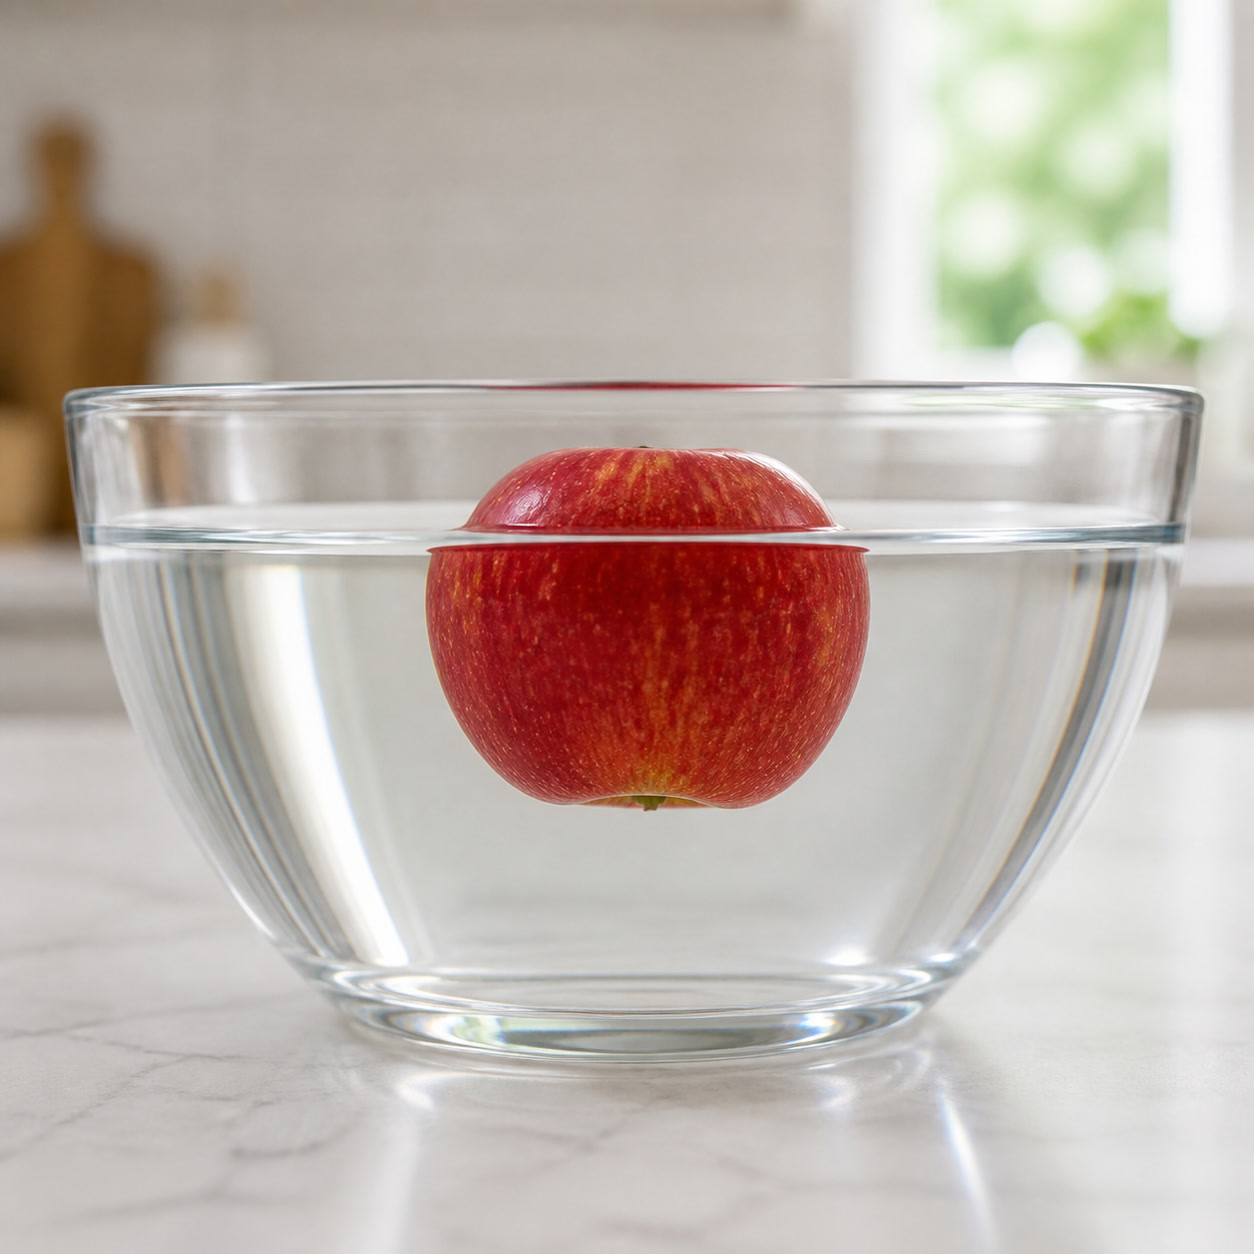
\includegraphics[width=0.42\linewidth]{images/book1/ai/g1-floating-apple.jpg}

{\small تفاحة تطفو في وعاء ماء: تركب منخفضة، وأكثر جسمها تحت السطح --- ومع ذلك فهي تطفو.}
\end{omfigure}

\section{الثقل ليس القصة كلها}

يتوقّع كثير من الناس أن ``الأشياء الثقيلة تغرق، والخفيفة تطفو''.
وللماء مفاجأة لهم.

\begin{example}[الجذع وقطعة النقود]\label{ex:g1:floating-and-sinking:log}
جذع شجرة ساقطة أثقل بكثير من أن ترفعه --- ومع ذلك \omterm{def:g1:floating-and-sinking:words}{يطفو} نازلًا مع
النهر. وقطعة نقود صغيرة أخفّ من قطعة بسكويت --- ومع ذلك تغرق في
الحال. إذن لا يمكن أن يكون الثقل والخفّة هما القاعدة كلها: فالجذع
الضخم \omterm{def:g1:floating-and-sinking:words}{يطفو} بينما تغرق القطعة الصغيرة.
\end{example}

\begin{example}[المادة هي التي تحسم]\label{ex:g1:floating-and-sinking:stuff}
عُد إلى لعبة التصنيف: طفت الملعقة البلاستيكية وغرقت المعدنية، مع
أن لهما الشكل نفسه والعمل نفسه. والذي صنع الفرق هو \emph{المادة}
التي صُنعتا منها --- فالخشب والفلّين وأكثر اللدائن موادّ طافية؛
والمعدن والحجر والزجاج موادّ غارقة. والشيء يتصرّف عادةً تصرّف
مادته: فالخشب \omterm{def:g1:floating-and-sinking:words}{يطفو}، غصينًا كان أم جذعًا كاملًا.
\end{example}

\begin{remark}[قليل من الغموض]\label{rem:g1:floating-and-sinking:why}
\emph{لماذا} \omterm{def:g1:floating-and-sinking:words}{يطفو} الخشب \omterm{def:g1:floating-and-sinking:words}{ويغرق} المعدن؟ ذلك سؤال حقيقي، وجوابه
الكامل من كنوز هذا المنهاج --- فهو يحتاج إلى أفكار تأتي في سنوات
لاحقة. أما الآن فنجمع ملاحظات جيدة؛ وسيجدنا ``اللماذا'' مستعدّين.
\end{remark}

\section{الماء يدفع من تحت}

\begin{example}[جرّب: ادفع الكرة تحت الماء]\label{ex:g1:floating-and-sinking:push}
خذ كرة طافية في حوض الحمّام وادفعها على مهل تحت الماء براحة يدك.
أتحسّ بذلك؟ الماء يردّها إلى الأعلى، وبقوة أشدّ كلما دفعتها أعمق
--- وإن انزلقت يدك قفزت الكرة خارجة من الماء. فالماء لا
\emph{يدع} الطافيات تستقرّ في أعلاه فحسب: بل يحملها حملًا، كما
تحمل يداك رضيعًا.
\end{example}

\begin{omfigure}
\begin{tikzpicture}[scale=0.85]
  \draw[thick] (0,0) -- (0,3.4) (0,0) -- (6.5,0) (6.5,0) -- (6.5,3.4);
  \draw[omDef, thick] (0,2.7) -- (6.5,2.7);
  \fill[omDef, opacity=0.15] (0,0) rectangle (6.5,2.7);
  \draw[thick, fill=white] (3.2,1.5) circle (0.6);
  \node[font=\small] at (3.2,1.5) {كرة};
  \draw[-Stealth, very thick, omThm] (3.2,3.3) -- (3.2,2.25);
  \node[right, font=\small, omThm] at (3.35,2.9) {يدك تدفع إلى الأسفل};
  \draw[-Stealth, very thick, omDef] (3.2,0.35) -- (3.2,0.85);
  \node[right, font=\small, omDef] at (3.35,0.55) {والماء يدفع إلى الأعلى};
\end{tikzpicture}

{\small كرة ممسوكة تحت الماء: يدك تدفع إلى الأسفل، والماء يدفع
إلى الأعلى. أفلتها، فيغلب دفع الماء.}
\end{omfigure}

\begin{example}[قارب المعجونة]\label{ex:g1:floating-and-sinking:boat}
دحرج قطعة من معجونة اللعب حتى تصير كرة وألقها في الماء: تغرق ---
فالمعجونة مادة غارقة. والآن خذ القطعة \emph{نفسها} وشكّلها وعاءً
صغيرًا بجوانب مرتفعة، وضعها برفق على الماء: تطفو! المادة نفسها،
والقطعة نفسها --- ولم يتغيّر إلا الشكل. فالشكل العريض المجوّف يعطي
الماء مساحة أكبر يدفع عليها. وهذا سرّ السفن العظيمة: المعدن مادة
غارقة، لكن بدن السفينة المعدني مشكّل كوعاء ضخم مجوّف.
\end{example}

\begin{omfigure}
\begin{tikzpicture}[scale=0.85]
  \draw[thick] (0,0) -- (0,2.6) (0,0) -- (4.6,0) (4.6,0) -- (4.6,2.6);
  \draw[omDef, thick] (0,2.0) -- (4.6,2.0);
  \fill[omDef, opacity=0.15] (0,0) rectangle (4.6,2.0);
  \fill[omThm] (2.3,0.35) circle (0.35);
  \node[below, font=\small] at (2.3,-0.2) {كرة معجونة: تغرق};
  \draw[thick] (6.4,0) -- (6.4,2.6) (6.4,0) -- (11,0)
    (11,0) -- (11,2.6);
  \draw[omDef, thick] (6.4,2.0) -- (11,2.0);
  \fill[omDef, opacity=0.15] (6.4,0) rectangle (11,2.0);
  \draw[thick, omThm, fill=white]
    (7.9,2.25) -- (8.1,1.75) -- (9.3,1.75) -- (9.5,2.25);
  \node[below, font=\small] at (8.7,-0.2) {القطعة نفسها وعاءً: تطفو};
\end{tikzpicture}

{\small قطعة معجونة واحدة، وشكلان، ومصيران. فشكل الوعاء المجوّف
يعطي الماء مساحة أكبر يحمل عليها.}
\end{omfigure}

\section{تمارين}

\begin{exercise}[$\star$]\label{exo:g1:floating-and-sinking:1}
صنّف إلى طافيات وغارقات: فلّينة؛ \ مفتاح؛ \ غصين يابس؛ \ كرة
زجاجية؛ \ بطّة بلاستيكية؛ \ حجر.
\end{exercise}

\begin{exercise}[$\star$]\label{exo:g1:floating-and-sinking:2}
في \cref{met:g1:floating-and-sinking:test}، لماذا يجب أن تضع الجسم
على الماء برفق بدل أن تقذفه فيه؟
\end{exercise}

\begin{exercise}[$\star$]\label{exo:g1:floating-and-sinking:3}
قبل الاختبار تتوقّع نورة: ``ستطفو الملعقة المعدنية لأن الملاعق
تطفو.'' ماذا حدث في لعبة التصنيف؟ وإلى ماذا ينبغي أن تنظر نورة بدل
عمل الشكل: المادة أم الاسم؟
\end{exercise}

\begin{exercise}[$\star$]\label{exo:g1:floating-and-sinking:4}
اذكر شيئًا ثقيلًا \omterm{def:g1:floating-and-sinking:words}{يطفو}، وشيئًا خفيفًا \omterm{def:g1:floating-and-sinking:words}{يغرق}. ماذا يبيّن هذا عن
التوقّع القائل ``الأشياء الثقيلة تغرق''؟
\end{exercise}

\begin{exercise}[$\star$]\label{exo:g1:floating-and-sinking:5}
الغصين \omterm{def:g1:floating-and-sinking:words}{يطفو}. فهل \omterm{def:g1:floating-and-sinking:words}{يطفو} جذع شجرة كامل أيضًا؟ وأيّ مثال من الفصل
يساعدك على الجواب؟
\end{exercise}

\begin{exercise}[$\star$]\label{exo:g1:floating-and-sinking:6}
ادفع كرة طافية تحت الماء في حوض الحمّام ثم أفلتها. بمَ تحسّ أثناء
الدفع، وماذا تفعل الكرة حين تفلتها؟
\end{exercise}

\begin{exercise}[$\star$]\label{exo:g1:floating-and-sinking:7}
السفن مصنوعة من المعدن، والمعدن مادة غارقة. فأيّ شكل ينقذ
السفينة؟ وأيّ تجربة في الفصل تبيّن ذلك؟
\end{exercise}

\begin{exercise}[$\star$]\label{exo:g1:floating-and-sinking:8}
اختبر وقت الحمّام: أتطفو قنّينة ماء ممتلئة مغلقة أم تغرق؟ وماذا
عن القنّينة نفسها فارغة بغطائها؟ قل توقّعك أولًا، ثم جرّب.
\end{exercise}

\begin{exercise}[$\star\star$]\label{exo:g1:floating-and-sinking:9}
قارب ليو المصنوع من المعجونة \omterm{def:g1:floating-and-sinking:words}{يطفو} طفوًا جميلًا --- حتى يعصره
فيعيده كرة، \omterm{def:g1:floating-and-sinking:words}{فيغرق}. يقول ليو: ``تعب الماء من حمله.'' أعطِ تفسيرًا
أفضل مستعينًا بما في \cref{ex:g1:floating-and-sinking:boat}.
\end{exercise}
